\documentclass[a4paper]{article}

\usepackage[english]{babel}
\usepackage[utf8]{inputenc}
\usepackage{amsmath}
\usepackage{graphicx}
\usepackage[colorinlistoftodos]{todonotes}

\title{Faster R-CNN}

\author{Christian Dingkuhn\\Matthias Greshake\\Yan-Frederic Thorsting}

\date{\today}

\begin{document}
\maketitle

\begin{abstract}
Object detection is a computer technology prominent in the fields of computer vision and image processing. It thus does not come as a surprise that research in object detection is critical in the development of technologies that involves face detection and pedestrian detection, among other domains. The \emph{Regional Convolutional Neural Network} (R-CNN) \cite{rcnn} is an early attempt to achieve object detection through the use of neural networks, it has since then been supplanted by the \emph{Spatial Pyramid Pooling network} (SPPnet) \cite{sppnet} or improved into the \emph{Fast R-CNN} \cite{fastrcnn}, both in terms of speed and accuracy. In this work, we introduce a "toy"-size implementation of more recent \emph{Faster R-CNN} of Ren et al. (2016) \cite{fasterrcnn}, which combines the so called \emph{Region Proposal Network} (RPN) \cite{fasterrcnn} with the Fast R-CNN for even better running time and accuracy score.
\end{abstract}

\section{Introduction}

Object detection being used in a wide range of domains, from face recognition to tracking a ball in a football match, developing fast and accurate methods to achieve it is therefore critical to the progress in the aforementioned domains.

The problem of object detection can be split into two smaller ones. The localization problem consists of localizing objects in the image, whereas assigning labels to the found objects amounts to solve the classification problem. Localization is especially important when the input image possibly contain more than one object. Without first localizing potential candidates, a traditional CNN would get confused with the multiple labels during the training, and as a result it may assign the wrong label to an object that just happened to frequently co-occur in the training data with the object to which that label actually corresponds. For example,  if a CNN is trained to recognize the object banana in an image, but in the training data bananas often co-occur with grocery bags, the CNN once trained may start to classify images featuring grocery bags as featuring bananas even though they may actually contain no banana at all.

Furthermore, localization is achieved by selecting the \emph{Region of Interests} (RoIs) on the input image that have a high "objectness" score. Earlier version of the R-CNN use either \emph{Selective Search} (SS), which greedily merges superpixels based on engineered low-level features \cite{ss}, or \emph{Edge Boxes} (EB), which use the number of contour wholly contained in a bounding box as object indicator \cite{eb}, to generate the RoIs. In a CPU implementation, SS takes 2 s/img, whereas EB takes 10$\times$ times less this value. The \emph{Region Proposal Network} (RPN) of the Faster R-CNN on the other hand achieves localization at nearly no cost (10 ms/img) by taking advantage of the GPU and sharing convolutions at test-time \cite{fasterrcnn}. The difference between the R-CNN and the Fast R-CNN in terms of object localization is that the former runs a CNN on top of each RoI, whereas the latter performs the feature extraction before generating the RoIs, thus running only one CNN over the entire image instead of many ($\sim$2,000) \cite{fastrcnn}. By doing so, the Fast R-CNN actually shares computation and greatly reduces the running time of the algorithm. For further processing of the RoIs in the Fast R-CNN, these are all resized and reshaped to the same size and form in the next (pooling) layer \cite{fastrcnn}.

As for classification, the output of the multiple CNNs (for the R-CNN) or that of the resized and reshaped RoIs (for the Fast R-CNN) are fed into \emph{fully connected} (fc) layers where they are classified by a SVM (for the R-CNN) or a softmax function (for the Fast R-CNN). From that point on, depending on the classifier's output, linear regression is applied to the RoIs' bounding boxes with high objectness score to refine their position \cite{fastrcnn}.

All in all, the main difference between the Fast R-CNN and the Faster R-CNN is the latter's use of a RPN for localization instead of a SS or a EB. In the following section we will thus introduce and explain our own implementation of both the RPN and the Fast R-CNN, followed by the training of this Faster R-CNN on a toy problem. A third section will be on the different experiments we conducted with this Faster R-CNN. And last and not least, the fourth section of this paper will be to discuss the results of the experiments, the performance of the Faster R-CNN and how it could possibly be improved.

\section{Data and Model Implementation}

\subsection{Data Generation}
We used 150 $256 \times 256 \times 1$ images. Those images were automatically generated by randomly putting 2 to 4 randomly drawn images from the MNIST database together on an unified black background. The MNIST numbers were randomly distributed on each individual images and could possibly overlap. It was necessary to replicate the $256 \times 256$ values onto three apparent color channels to fit the expected input tensors dimensionality of the used pretrained VGG. Furthermore, each MNIST collage had assigned to it a list of the form $[img_1, img_2, img_3, img_4]$, with each element corresponding to a seven-tuple of the form ($mnist\_number$, $x_{center}$, $y_{center}$, $w$, $h$, $angle$, $scale$). Each of these seven-tuples represent a MNIST image on the collage, with $mnist\_number$ standing for the represented number, $x_{center}$ and $y_center$ for the $x$ and $y$ coordinates of the image on the collage respectively, $w$ for the width of the image, $h$ for the height of the image, $angle$ for the angle of the image, and $scale$ for the scale of the image.

\subsection{Pretrained VGG-16}
This implementation of the Faster R-CNN consists of a fixed VGG-16 model pre-trained on ILSVRC-2012, and custom-made RPN and Fast R-CNN. Code is available at https://github.com/YFSTH/Tensorflow-Project.

We fed the collages to the VGG-16, collected the ReLU-processed output of the last convulotional (conv) layer, which was a feature tensor of shape $1 \times 16 \times 16 \times 512$ and used it as the input of our RPN.

\subsection{Region Proposal Network}
As a localizer for the Faster R-CNN, the RPN takes an image (of any size) as input and outputs a set of rectangular RoIs, each with an objectness score. Unlike with the Faster R-CNN of Ren et al. \cite{fasterrcnn} however, this network will not be sharing the convolution with the Fast R-CNN in an end-to-end manner.

To generate the RoIs, a small network is slid over the $16 \times 16 \times 512$ feature tensor output by the first conv layer. This network is fully connected to a $3 \times 3$ spatial window of the input conv feature map. Each sliding window is mapped to a 512-dimension vector. This vector is fed into two sibling fully-connected layers---a $1 \times 1 \times 512 \times 36$ box-regression layer and a $1 \times 1 \times 512 \times 18$ box-classification layer. The last dimension of the box-regression layer corresponds to the $x$ (entries 1-9) and $y$ (entries 10-18) coordinates, the width (entries 19-27), and to the height (entries 28-36) of the RoIs; whereas the last dimension of the box-classification layer corresponds to the objectness score (entries 1-9) and non-objectness score (entries 10-18) of the anchors. Because the mini-network operates in a sliding-window fashion, the fully-connected layers are shared across all spatial locations. ELUs are applied to the output of the $3 \times 3$ conv layer \cite{fasterrcnn}.

\paragraph{Translation-Invariant Anchors}
As it has been previously been hinted, there are 9 anchors for each sliding position. In Ren et al. (2016) \cite{fasterrcnn} they represent 3 scales and 3 aspect ratios, we however opted for 9 identical anchors instead, because all MNIST images were square-shaped and else it would have been difficult to yield enough positive anchors for further processing. Thus, for a conv feature map of a size $16 \times 16$, there are $2304$ anchors in total. An important property of this approach is that it is \emph{translation invariant} \cite{fasterrcnn}, both in terms of the anchors and the functions that compute proposals relative to the anchors.

\paragraph{A Loss Function for Learning Region Proposals}
For the RPN training, a binary class label (of being an object or not) is assigned to each anchor. A positive label is assigned to two kinds of anchors: (i) if a ground-truth box has no anchor it has an \emph{Intersection-over-Union} (IoU) bigger or equal than 0.7 then the anchor/anchors with the highest IoU with the box is assigned to it, or (ii) else if an anchor has an IoU bigger than 0.7 with any ground-truth box then it is assigned to the box it has the highest IoU with (under the condition that no box was already assigned by the first rule). Note that a single ground-truth box may assign positive labels to multiple anchors, but maximally one ground-truth box will be assigned to a single anchor \cite{fasterrcnn}. A negative label is assigned to a non-positive anchor if its IoU ratio is lower than 0.3 for all ground-truth boxes. If an anchor is neither positive or negative it does not contribute to the training objective \cite{fastrcnn}.
\\
\\
For this implementation, we adopt the single image loss function of Ren et al. (2016) \cite{fasterrcnn}:

$$L({p_i},{t_i}) = \frac{1}{N_{cls}} \sum_i L_{cls} (p_i,p_i^*) + \lambda \frac{1}{N_{reg}} \sum_i p_i^* L_{reg} (t_i,t_i^*).$$

\noindent Here, $i$ corresponds to the index of an anchor and $p_i$ to the predicted probability of an anchor $i$ being an object. $p_i^*$ corresponds to the ground-truth label and is 1 if the anchor is positive, and 0 if it is negative. $t_i$ corresponds to a vector representing the 4 parameters of the predicted bounding box, and $t_i^*$ is that of the ground-truth box associated with a positive anchor. We used cross-entropy as the classification loss $L_{cls}$. As the regression loss, we used the smooth $L_1$ loss applied by Girshick (2015) \cite{fastrcnn}. This loss can only be calculated for positive anchors because only to them a ground-truth box was assigned. The normalized the regression error by dividing it by $16 \times 16 \times 9$ (which is equal to the number of anchors per collage) and the classification error we divide it by the number of anchors we used to calculate it. $\lambda$ as in Ren et al. (2016) was set to 10 to roughly equalize the contribution of both error terms to the overall error \cite{fasterrcnn}.
\\
\\
Like in Ren et al. (2016) \cite{fasterrcnn}, the parameterizations for regression of the 4 coordinates is adopted following Girshick et al. (2014) \cite{rcnn}:

$$t_x = (x - x_a)/w_a, t_y = (y - y_a)/h_a, t_w = log(w/w_a), t_h = log(h/h_a),$$
$$t_x^* = (x^* - x_a)/w_a, t_y^* = (y^* - y_a)/h_a, t_w^* = log(w^*/w_a), t_h^* = log(h^*/h_a),$$
\\
where $x$, $y$, $w$, and $h$ corresponds to the parameters of the box center, width and height. Whereas $x$, $x_a$, and $x^*$ correspond to the predicted box, the anchor box, and the ground-truth box respectively (the same goes for $y$, $w$ and $h$) \cite{fasterrcnn}.

In this method, the features used for regression are of the same size ($3 \times 3$) on the feature maps \cite{fasterrcnn}.

\subsection{Fast R-CNN}
The Fast R-CNN requires equally shaped regions as inputs to its feed-forward layers. To achieve this, a method called \emph{RoI pooling} \cite{fastrcnn} is applied: differently shape region proposal are mapped to an always equally shaped region which represents the input to the subsequent layer of the Fast R-CNN \cite{fastrcnn}. We used the following algorithm to perform RoI pooling. (i) We upscaled the proposal by a factor equal to the targeted RoI pooling output size without applying any smoothing (basically just stretching the region's pixels), (ii) then we used a max pooling kernel of a shape equal to the shape of the unprocessed proposal and strides equal to the width or height respectively of this proposal. This procedure resulted in a RoI pooling output of the desired shape \cite{fastrcnn}.
\\
\\
A Fast R-CNN network takes as input an entire image and a set of object proposals. The network first processes the whole image with several conv and max pooling layers to produce a conv feature map. Then, for each RoI a pooling layer extracts a fixed-length feature vector from the feature map. Each feature vector is fed into a sequence of fc layers that finally branch into two sibling output layers. Like the RPN, the Fast R-CNN has two heads, one for regressing the proposal parameters onto the ground-truth box parameters and a classification head to determine the probability for the proposal belonging to one of the 10 classes \cite{fastrcnn}.

As for the RPN, a multi-task loss is applied, which simply consist of the sum of the cross-entropy classification loss and the smooth $L_1$ bounding-box regression loss.

$$L(p,u,t^u,v) = L_{cls} + \lambda[u \geq 1]L_{reg}(t^u,v),$$

\noindent As in the implementation of Girshick (2015), $\lambda$ was set to 1 and the regression loss was normalized by the total amount of anchors per image, equaling $16 \times 16 \times 9 = 2304$ anchors, to equalize the contribution of both loss components \cite{fastrcnn}.

\subsection{Training}

We applied a two-steps training procedure: (i) we fed single collages to the VGG-16, collected the output of the last conv layer and fed this to the RPN to predict proposal parameters and objectness score for each positive anchor. In total we used 150 collages and fed them each 12 times, resulting in 1800 iterations. Then we used the Adam-optimizer with default settings ($\beta_1 = 0.9$, $\beta_2 = 0.999$, $y = 1e-8$) a piece-wise learning rate decay (learning rate of $1E-3$ until iteration 1,200, $1E-4$ until iteration 1,600 and after that, until the last iteration of 1,800 a learning rate of $5E-6$). (ii) We fed selected proposals with readjusted parameters such that the proposals are not outside the image frame to the RoI pooling layer of the Fast R-CNN and try to train the Fast R-CNN with Adam-optimizer using the default setting mentioned above with a learning rate of 0.01 and 0.001, however these attempts were not successful and we unfortunately ran out of time.

\section{Training Results}

As it can be partly seen in Figure 1, both the classification loss as well as the overall loss decrease rapidly during the early iterations, being slightly above 0. Interestingly, the regression loss was very low from the beginning and very close to 0, however decrease even further during the iterations.
Also, the objectness classification accuracy showed a rapid improvement approaching 100\% during early iteration.

\begin{figure}
\centering
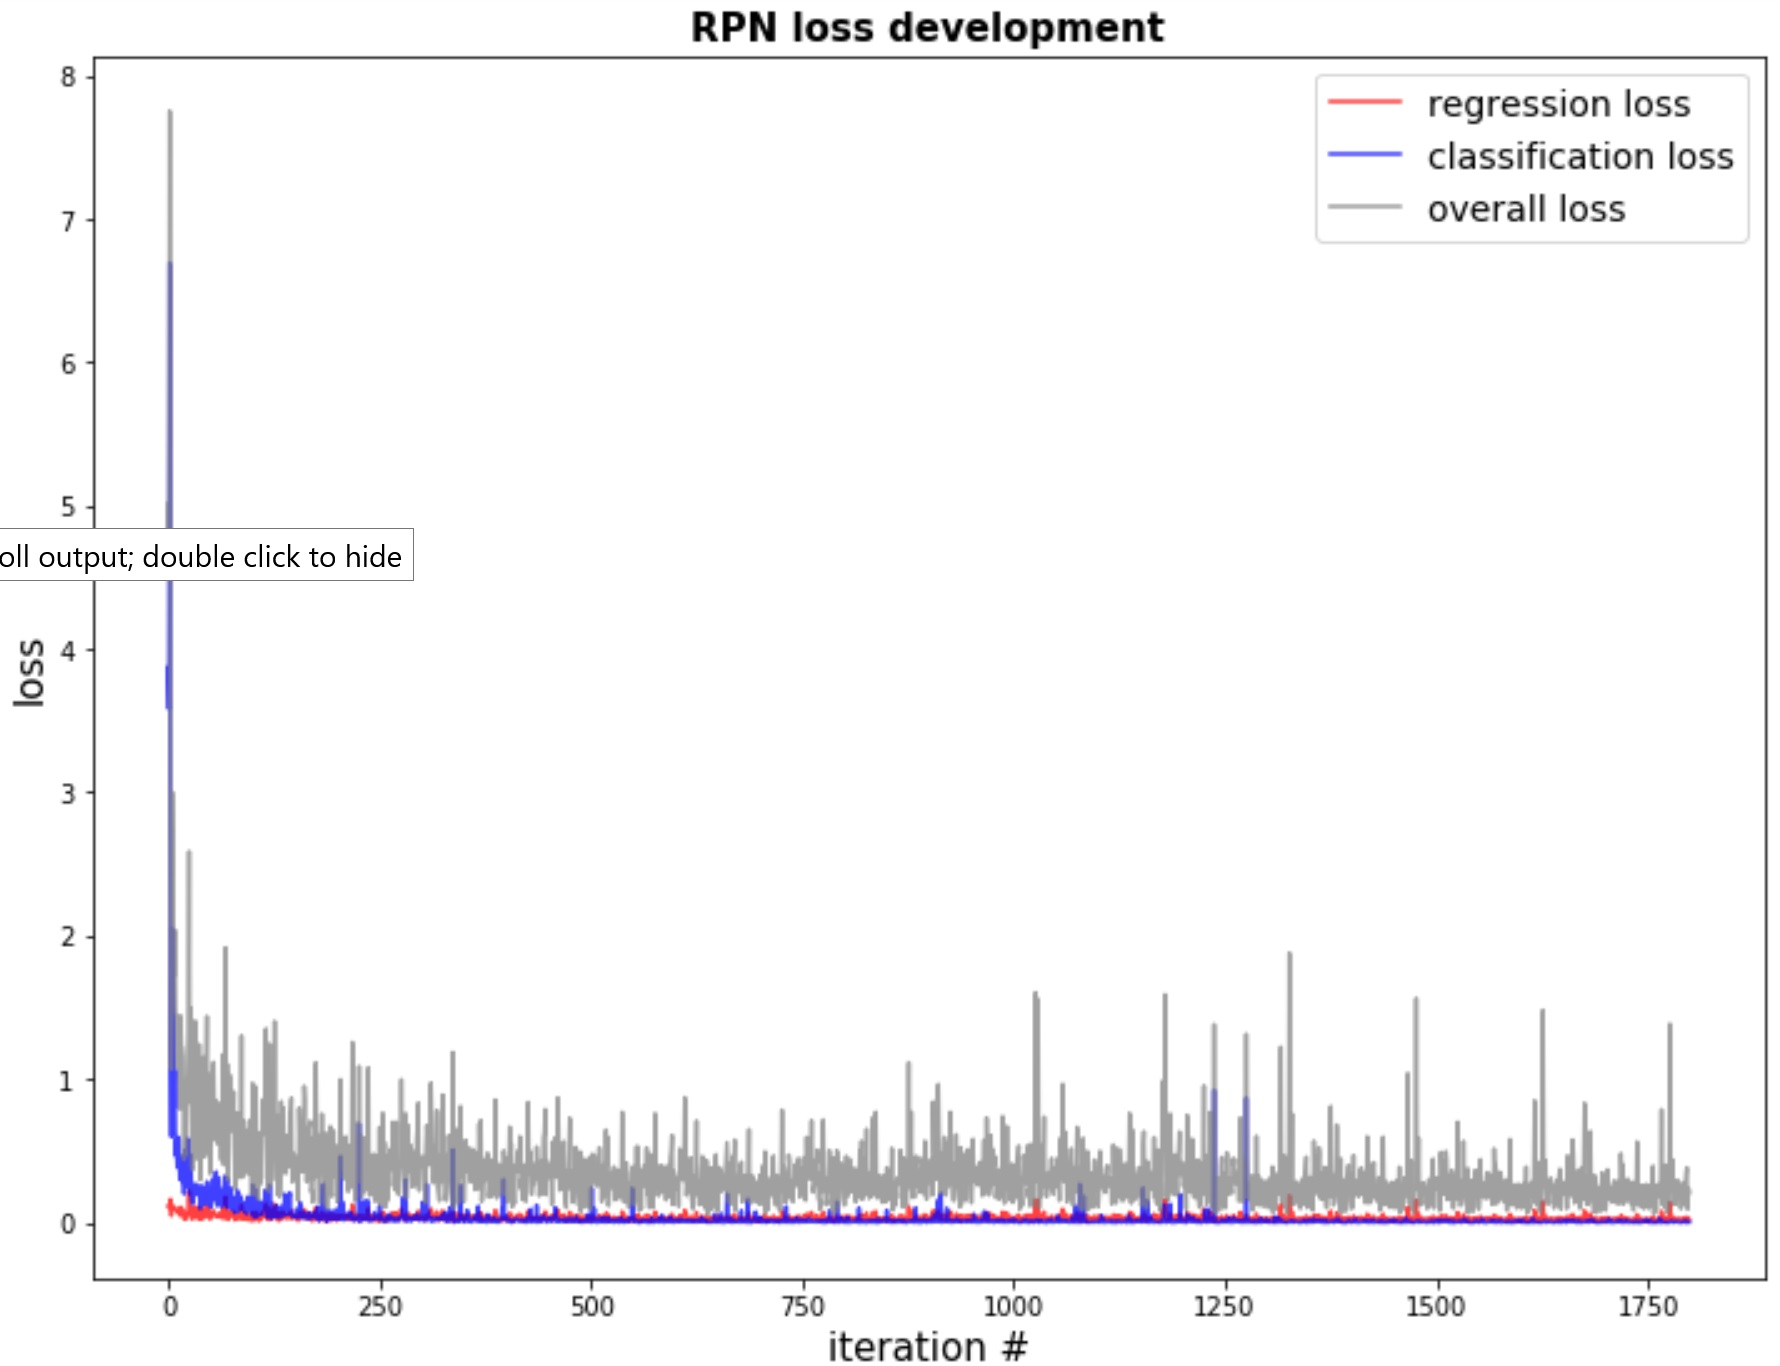
\includegraphics[width=0.8\textwidth]{rpn_loss_development.jpg}
\caption{\label{fig:rpn_loss_development}Note that loss measures for regression and classification differ. Cross-entropy is used for classification, whereas for regression the smooth $L_1$ loss is applied, and the overall loss is a weighted sum of both.}
\end{figure}

\begin{figure}
\centering
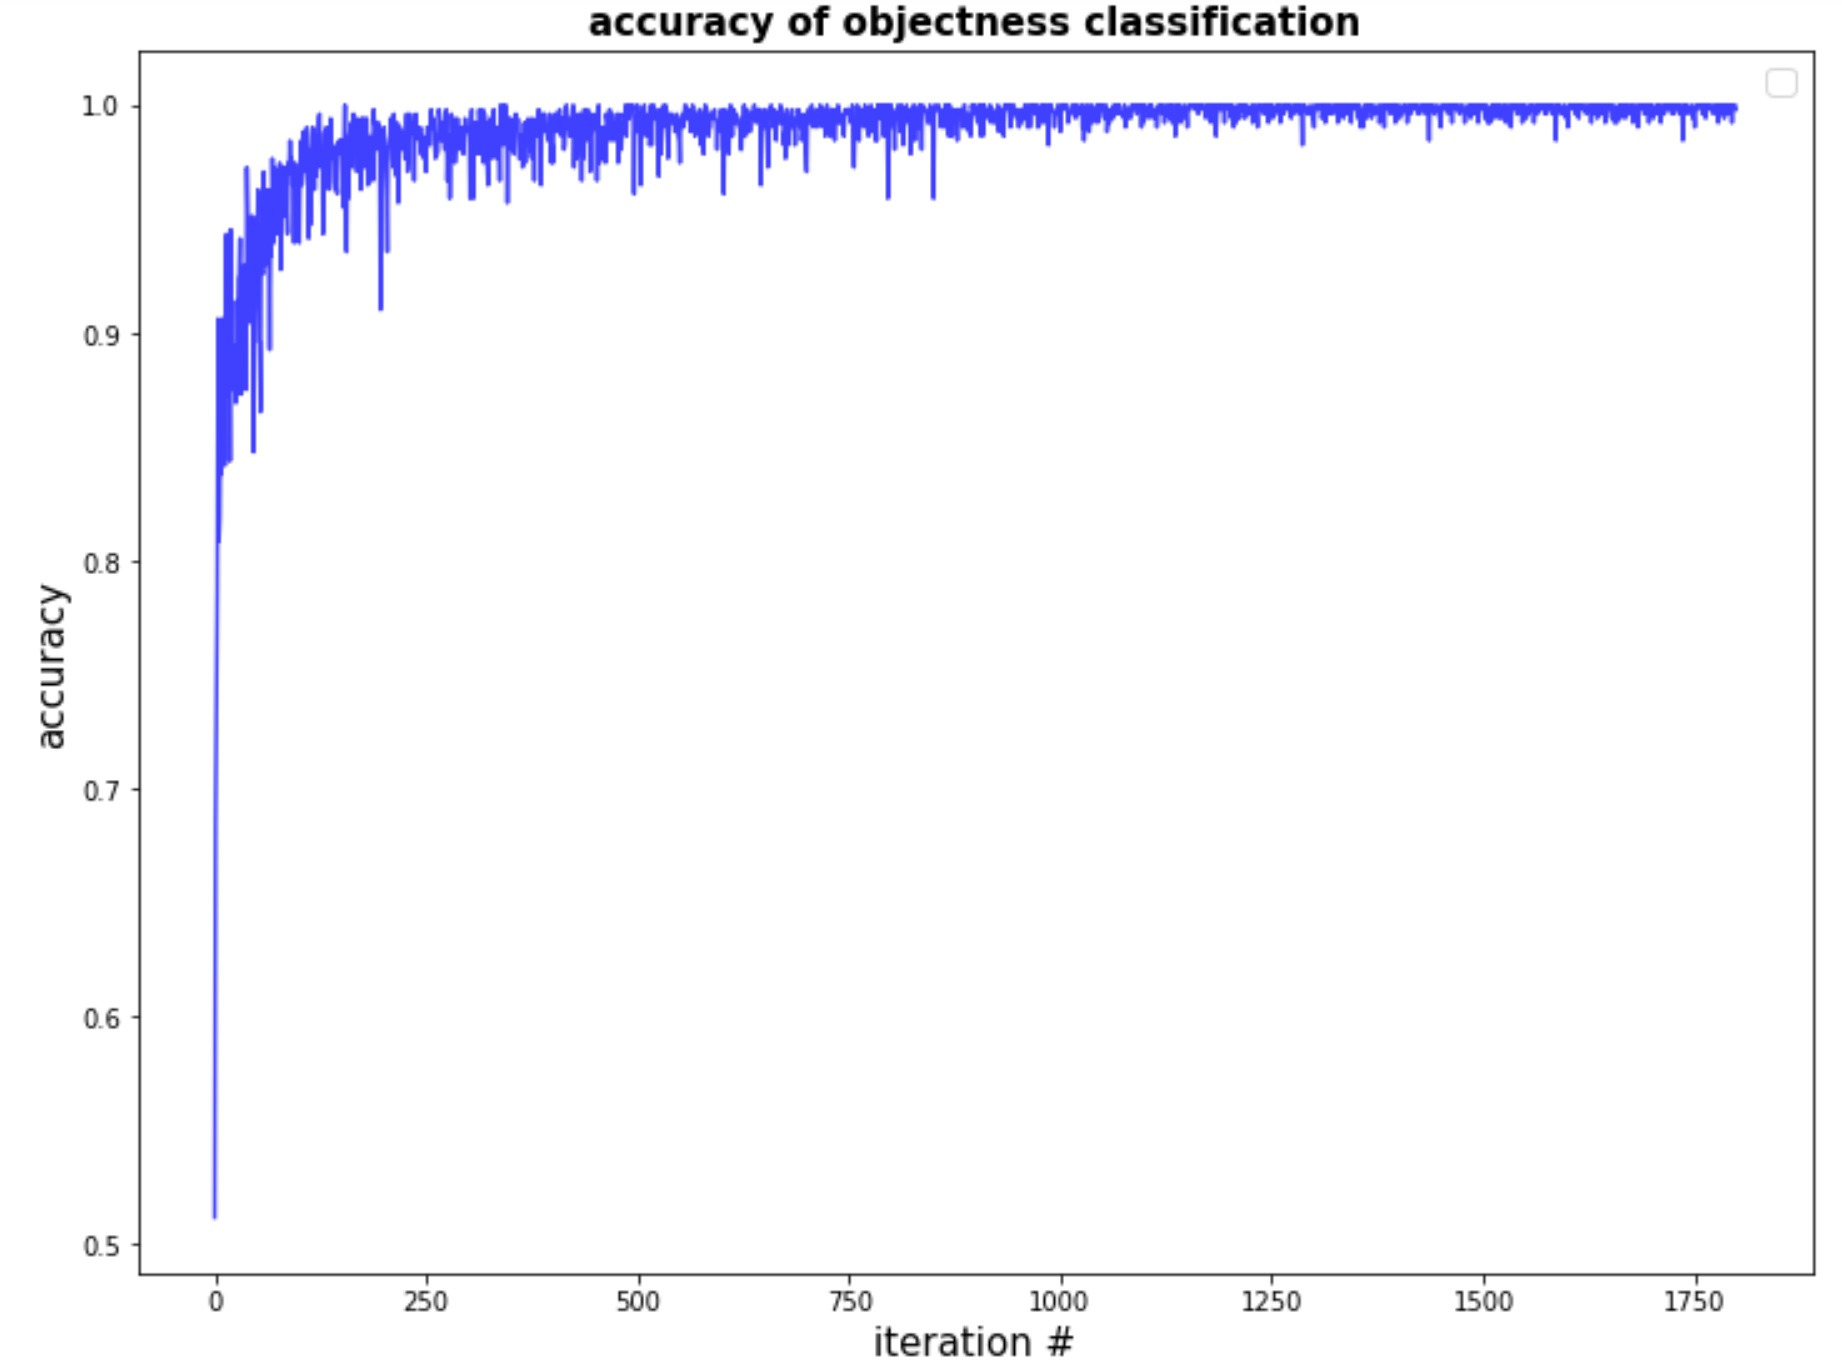
\includegraphics[width=0.8\textwidth]{rpn_accuracy.jpg}
\caption{\label{fig:rpn_accuracy} Accuracy of the RPN objectness classification vs. number of iteration of the box-classification layer.}
\end{figure}

\newpage

\section{Discussion}

The rapid improvement of the losses and the accuracy might be due to the simple task of just predicting the region of MNIST images and their presence on a black background. Fitting to that, the proposed regions captured the MNIST images regions often quite well (not shown in the results), however the very low initial value of the regression loss hints to an unsolved issue.
On the \emph{PASCAL VOC 2012} benchmark \cite{voc} with the very deep convolutional neural network \emph{VGG-16} \cite{vgg}, the Faster R-CNN of Ren et al. (2016) achieved 198 ms/img and 70.4\% \emph{mean Average Precision} (mAP) \cite{fasterrcnn}. It represents a net improvement over the earlier methods, with the R-CNN of Girshick et al. (2014) scoring 62.4\% mAP \cite{fastrcnn}, and the Fast R-CNN of Girshick (2015) reaching 1830 ms/img and 68.4\% mAP \cite{fasterrcnn}.
Unfortunately, due to time constraints, we were not able to implement a working version of the Fast R-CNN, which leaves open a lot of room for further improvements.

\newpage

\begin{thebibliography}{9}
\bibitem{rcnn}
R. Girshick, J. Donahue, T. Darrell, and J. Malik. Rich feature hierarchies for accurate object detection and semantic segmentation. In \emph{CVPR}, 2014.
\bibitem{sppnet}
K. He, X. Zhang, S. Ren, and J. Sun. Spatial pyramid pooling in deep convolutional networks for visual recognition. In \emph{ECCV}, 2014.
\bibitem{fastrcnn}
R. Girshick. Fast R-CNN. \emph{arXiv:1504.08083}, 2015.
\bibitem{fasterrcnn}
S. Ren, K. He, R. Girshick, and J. Sun. Faster R-CNN: Towards Real-Time Object Detection with Region Proposal Networks. In \emph{arXiv:1506.01497v3}, 2016.
\bibitem{voc}
M. Everingham, L. Van Gool, C. K. I. Williams, J. Winn, and A. Zisserman. The PASCAL Visual Object Classes Challenge 2007 (VOC2007) Results, 2007.
\bibitem{vgg}
K. Simonyan and A. Zisserman. Very deep convolutional networks for large-scale image recognition. In \emph{ICLR}, 2015.
\bibitem{ss}
J. R. Uijlings, K. E. van de Sande, T. Gevers, and A.W. Smeulders. Selective search for object recognition. emph{IJCV}, 2013.
\bibitem{eb}
C. L. Zitnick and P. Doll\'ar. Edge boxes: Locating object proposals from edges. In \emph{ECCV}, 2014.

\end{thebibliography}
\end{document}